
\begin{infocard}{Volumen de un prisma recto}
    El volumen de un prisma recto de altura $h$, y cuyo polígono base tiene un área $A_b$, se obtiene mediante la expresión:
    \[
        V = A_b h
    \]
    \begin{figure}[H]
        \centering
        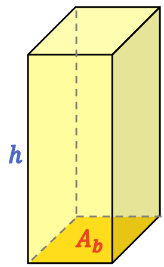
\includegraphics[width=0.3\textwidth]{../images/20230319192423}
        \caption{}
        \label{fig:20230319192423}
    \end{figure}
    
    Si el polígono base es un polígono regular (todos sus lados iguales), entonces:
    \[
        V  = \dfrac{nLah}{2}
    \]
    donde $A_b$ es el área del polígono regular de la base, $P$ es el perímetro; $a$, la apotema; $n$, el número de
    lados; $l$, la medida del lado y $h$, la altura.
\end{infocard}



